%% This is a sample file demonstrating the use of IJCAS.cls,
%% which is for the IJCAS (International Journal of Control, Automation, and Systems).
%%
%% 2004/03/08 by Karnes Kim
%% 2011/07/26 by CDSL, SNU
%%
%% Support sites: http://www.ijcas.com
%%
%% This code is offered as-is - no warranty - user assumes all risk.
%% Free to use, distribute and modify.
%%

%% The IJCAS class supports two column page basically. 
%%So, you need not use two column option or command.
\documentclass{IJCAS}


%% include the useful LaTeX packages:
\usepackage{url}
\usepackage{array,tabularx}
\usepackage{multicol} 


\usepackage{amsmath,amssymb,amsfonts}
\usepackage{tabularx}
\usepackage[utf8]{inputenc} % allow utf-8 input
\usepackage[T1]{fontenc}    % use 8-bit T1 fonts
\usepackage{url}            % simple URL typesetting
\usepackage{booktabs}       % professional-quality tables
\usepackage{amsfonts}       % blackboard math symbols
\usepackage{nicefrac}       % compact symbols for 1/2, etc.
\usepackage{microtype}      % microtypography
\usepackage{graphicx}
\usepackage{float}
\restylefloat{table}
\usepackage{hyperref}
\usepackage{multicol}
\usepackage{caption}
\usepackage{subcaption}
\usepackage{amsmath}
\usepackage{algorithm}
\usepackage{algpseudocode}
\usepackage{tikz}
\usetikzlibrary{trees}
\usepackage{listings}
\usepackage{array}
\usepackage{colortbl,hhline}
\usepackage{color}
\usepackage{multirow}
\usepackage{xcolor}

\DeclareMathOperator*{\argmax}{arg\,max}  % in your preamble
\DeclareMathOperator*{\argmin}{arg\,min}  % in your preamble

\usepackage{textcomp}

%\usepackage[retainorgcmds]{IEEEtrantools}
%\usepackage{bibentry}
\usepackage{xcolor,soul,framed} %,caption

\usepackage[noadjust]{cite}
%\usepackage{biblatex}
%\bibliographystyle{plain}

\usepackage[font=normalsize]{caption}
\captionsetup[figure]{font=normalsize}



%%%% Editorial Information
%% Authors do not have to modify this section.
\journalvolumn{VV}
\journalnumber{X}
\journalyear{YYYY}
\setarticlestartpagenumber{1}
%%%% End of Editorial Information

%The environment for theorem, lemma, remark, corollary, proposition, and definition are already defined.


%The following command is needed for line break of long equations.
\allowdisplaybreaks

\begin{document}
%% TITLE, AUTHOR, ABSTRACT, KEYWORDS

% the \title command
\title{Coaching with PID Controllers: Accelerate Reinforcement Learning with PID Coaches in the Pendulum Simulations}

% the \author command
\author{Zongqiang Pang*\orcid{}, Liping Bai\orcid{}, and Yang Yang\orcid{}
}%  <- don't remove this stop

% the abstract environment
\begin{abstract}
We propose a Proportional Integral Derivative (PID) controller-based coaching scheme to expedite reinforcement learning (RL). We demonstrate the feasibility and effectiveness of our approach in the inverted pendulum, inverted double pendulum simulation. Previous attempts to merge classical control with reinforcement learning focus on utilizing existing controllers as teachers to the RL agents, but they require high fidelity controllers and the benefit comes with an implicit cap on what is attenable by the RL agent. We ask if it is possible to accelerate RL with even a primitive hand-tuned PID controller and not inadvertently inflicting any limit to the RL agent. Instead of being teachers, the PID controllers function as coaches, whose job is not to provide templates to be imitated after but to be ready with necessary interventions. RL training can be expedited so long as the PID coaches can provide the appropriate assistance with a reasonable success rate. We validate our approach in the Mujoco Inverted Pendulum and Inverted Double Pendulum simulations. We conclude from the data that when the coaching structure between the PID controller and its respective RL agent is designed appropriately, the agent's training can be accelerated, yielding uncompromised training results. This is an important proof of concept that controller-based coaching can be a novel and effective paradigm for merging classical control with learning and warrants further investigations in this direction. All the code and data can be found at \href{https://github.com/BaiLiping/Coaching}{github/BaiLiping/Coaching}
\end{abstract}

% the keywords environment
\begin{keywords}
Reinforcement Learning, Control, Learning for Dynamic Control, L4DC
\end{keywords}

\maketitle

\makeAuthorInformation{

Zongqiang Pang, Liping Bai, Yang Yang are with the College of Automation \& College of Artificial Intelligence, Nanjing University of Posts and Telecommunications, Nanjing, Jiangsu,210000 China email:zqpang@njupt.edu.cn. 
* Corresponding author.
}
\runningtitle{2021}{Zongqiang Pang, Liping Bai, Yang Yang}{Manuscript Template for the International Journal of Control, Automation, and Systems: ICROS {\&} KIEE}{xxx}{xxxx}{x}

\section{Introduction}
Learning for Dynamic Control is an emerging field of research located at the interaction between classic control and reinforcement learning (RL). Although RL community routinely generate jaw-dropping results that seem out of reach to the control community\cite{Dao2020AdaptiveRL}\cite{Zheng2020BalanceCF}\cite{Xin2020RobustES}\cite{Dornheim2018ModelfreeAO}, the theories that undergird RL are as bleak as it was first introduced\cite{Bertsekas1996NeuroDynamicP}. Today, those deficiencies can be easily papered over by the advent of Deep Neural Networks (DNN) and ever faster computational capacities. However, for RL to reach its full potential, existing control theories and strategies have to be part of that new combined formulation.

There are three ways that classic control finds its way into RL. First, theorists who are well versed in optimization techniques and mathematical formalism can provide systematic perspectives to RL and invent the much needed analytical tools\cite{Han2020ActorCriticRL}\cite{Weinan2017APO}\cite{Dupont2019AugmentedNO}\cite{Betancourt2018OnSO}\cite{Nachum2020ReinforcementLV}\cite{Lv2019ApproximateOS}. Second, system identification researchers are exploring all possible configurations to combine existing system models with DNN and its variations\cite{Hewing2020LearningBasedMP}\cite{Mohan2020EmbeddingHP}\cite{Lusch2018DeepLF}\cite{Bai2019DeepEM}\cite{BelbutePeres2020CombiningDP}\cite{Oh2020DeepRB}\cite{Cheng2019OnorbitRU}. Third, proven controllers can provide data on successful control trajectories to be used in imitation learning, reverse reinforcement learning, and "human"-in-the-loop learning\cite{Knox2009InteractivelySA}\cite{Knox2010CombiningMF}\cite{Peng2018DeepMimicED}\cite{Peng2020LearningAR}\cite{Paine2018OneShotHI}\cite{Choi2017InverseRL}.

Our approach is an extension of the third line of research. We propose a coaching structure between the classical controllers and the RL agents. Professional athletes don't get where they are via trial-and-error. Their skillsets are forged through painstakingly designed coaching techniques. At the top level, a coach's objective is not to be a template for the athletes to imitate after, but rather is to facilitate data collection on critical states. 

Previous researches\cite{Xie2018LearningWT}\cite{Carlucho2017IncrementalQS}\cite{Pavse2020RIDMRI}\cite{Choi2017InverseRL} are about making a functioning controller works better. They require high-quality controllers to begin with, and the improvements brought about by the RL agents are merely icing on the cake. In addition, the controllers inadvertently impose limits on what can be achieved by the RL agents. If, unfortunately, a bad controller is chosen, then the RL training process would be hindered rather than expedited. 

\definecolor{airforceblue}{rgb}{0.36, 0.54, 0.66}
\definecolor{beaublue}{rgb}{0.74, 0.83, 0.9}

\begin{table}
\footnotesize
\caption{Performance of the PID controllers, as indicated by the average score over 10 episodes.}
\label{score_compare}
\centering
\begin{tabular}{ cccc }
\rowcolor{airforceblue}
Environment & PID Controller &Full Score &PID\slash Full Score \\
Inverted Pendulum & 240 & 1000& 24.0\%\\
\rowcolor{beaublue}

Double Pendulum & 1107 & 10000& 11.07\%\\
\end{tabular}
\end{table}

In our approach, the Coaches are PID controllers that can only score a fraction of what is available, as shown by Table \ref{score_compare}. Yet, even with such barely-functioning controllers, when appropriately structured, RL agent training acceleration is still observed in our experiments, as shown by Table \ref{episode_compare}. "Coaching" means the PID controller takes over when the RL agent deviated from the essential states. Our approach also differs from previous researches in one significant way: interventions from the coach are hidden from the RL agents and they are not part of the training data. We also restrain from reward engineering, such that we can be confident that the observed acceleration does not stem from other alterations. The implementations would be detailed in subsequent sections.




\begin{table}
\scriptsize
\caption{Comparison Between RL Agents Trained With and Without PID Coaches.}
\label{episode_compare}
\centering
\begin{tabular}{ cccccc }
\rowcolor{airforceblue}

Environment & Target & Measure & With PID & Without & Percentage\\
\rowcolor{airforceblue}

Name & Score & & Coach & Coach & Improvement \\
Inverted & 800& 5 Wins & 90 & 160& 43.8\% \\
Pendulum & &Average & 91 & 159& 42.8\%\\
\rowcolor{beaublue}
Double & 7000& 5 Wins & 1024 & 1909& 46.3\%\\
\rowcolor{beaublue}
Pendulum & &Average & 1391 & 2031& 31.5\%\\

\end{tabular}
\end{table}

In section II, we present the idea of controller-based coaching. In section III, we present the results of our experiments in the inverted pendulum and inverted double pendulum simulations. We conclude what we have learned and layout directions for further research in section IV.

\section{Methods}

Reinforcement Learning is the process of cycling between interaction with an environment and refinement of the understanding of that environment. RL agents methodically extract information from experiences, gradually bounding system models, policy distributions, or cost-to-go approximations to maximize the expected rewards along a trajectory. RL is an umbrella term that encompasses distinctive learning genres, which means updating parameters for the function approximators. A general taxonomy of RL is listed below:

Model-Based or Model-Free learning refers to whether or not learning is used to approximate the system dynamics function. If there is an explicit action policy, it is called on-policy learning. Otherwise, the optimal action would be implicitly captured by the Q value function, which would be called off-policy learning instead. Importance sampling allows "limited off-policy learning" capacity, which enables data reuse in a trusted region. Online learning means interleaving data collection and iterative network parameters update. Offline learning means the data is collected in bulk first, and then the network parameters are set with regression computation. Batch learning, as the name suggested, is in between online and offline learning. An agent would first generate data that fill its batch memory and then sample from the batch memories for iterative parameter update. Generate new data with the updated parameters. This taxonomy is somewhat outdated now. When Richard Sutton wrote his book\cite{Sutton1998IntroductionTR}, the algorisms he had in mind fall nicely into various categories, today, however, the popular algorisms would combine more than one route to derive superior performance and can't be pigeonholed.

A fundamental concept in RL is convergence through bootstrap: instead of asymptotically approaching a known target function, the bootstrap method converges to an assumed target first and then update the target assumption based on collected data. When evaluating estimation functions with belief rather than the real value, things could just run around in circles and never converge. Without any guidance, the RL agent would have explored all the possible states, potentially resulting in this unstable behavior. 

How to collect data in the most efficient manner (Exploration Exploitation Trade-off) and avoid the instability mentioned above in the bootstrap process is a primary focus of researchers. One such method is to give more weight to critical states. Not all observational states are created equal. Some are vital, while others have nothing to do with the eventual objective. For instance, in the inverted pendulum task, any states outside of the Lyapunov stability bounds should be ignored since they would lead to an episode's eventual termination anyway. 

There are statistical techniques to distinguish critical states from the non-essential ones, and imitation learning works by marking crucial states with demonstrations. However, the former approach is hard to implement, and the latter one requires high-quality controllers. Our proposed controller-based coaching method is easy to implement and does not have stringent requirements on the controllers it uses.

Controller-based coaching works by adjusting the RL agent's trajectory and avoid wasting valuable data collection cycle on the states that merely lead to eventual termination. When the agent is about to deviate from essential states, the controller will apply a force to nudge the agent back to where it should be, much like a human coach course-corrects on behalf of the athlete. 

Crucially, the agent is oblivious to this intervention step, and it would not be part of the agent's data. Even if the controller didn't adjust the agent to where it should be, it would not have mattered since the RL agent is headed towards an episode's termination. 

On the other hand, if the controller successfully adjusts the trajectory, the RL agent's next data collection cycle will be spent in a critical state. Therefore, all we require of the PID controller is a reasonable success rate in adjusting the RL agent's trajectory. We test our approach on four mujoco locomotion environments as a proof of concept, and in all four experiments, the hypothesized acceleration on RL training is observed.

\section{Experimental Results}
Mujoco physics engine\cite{6386109}, is one of many such simulation tools. We interface with it through a python wrapper provided by the OpenAI Gym\cite{Brockman2016OpenAIG}. We choose two environments for our experiments as a proof of concept: inverted pendulum, double inverted pendulum. 

Every environment comes with a set of predetermined rewards and maximum episode steps. We did not tinker with those parameters. The only change we made to each environment is a controller-based coach ready to intervene when the agent steps out of the predetermined critical states.

We use tensorforce's\cite{tensorforce} implementation of RL agents, specifically the Proximal Policy Optimization (PPO) agent because the learning curves generated by PPO agent are smoother, as shown by the spinning up\cite{SpinningUp2018} team. Our paper aims to indicate the controller-based coaching method's feasibility, and a smoother curve makes things easier. 

In this paper, human judgment is the basis for the determination of critical states. In future works, we would like to provide a more systematic process for critical states' demarcation. We will provide our reasonings when we discuss our experiments in each environment. 

Our experiments' code and data can be accessed via \href{https://github.com/BaiLiping/Coaching}{this depository}. The folders are named after each environment, and in each folder, you will find a data record, an RL agent record, a agent.json file that indicates all the hyperparameters for the RL agent, a Normal file that trains a RL agent without a PID coach, a Coached file which trains a RL agent with a PID coach, a PID file which is the PID controller. In the PIDvsRL folder, you will find all data and codes that generate the plots shown in the following section.

\subsection{Inverted Pendulum}
The observation space of the inverted pendulum environment is: [Cart Position on X-axis, Cart Velocity, Pole Angle, Pole Angular Velocity]. The continuous action space is an action ranging from -1 to 1, where -1 means the actuator moves the cart to the left with maximum power and 1 means the actuator moves the cart to the right with full force. The maximum episode step number is 1000. The terminal state for the inverted pendulum is an angle of absolute value greater than 0.2 radius. The reward is 1 for each non-terminal step and 0 for the terminal step. 

\begin{figure}[H]
  \centering 
  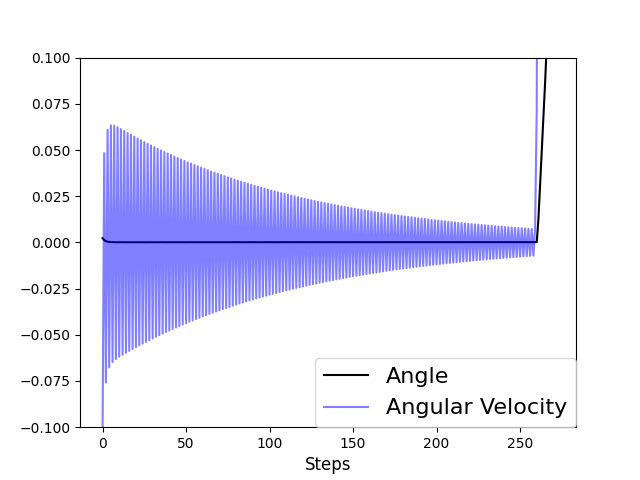
\includegraphics[width=0.3\textwidth]{ip_PID}
  \caption{Inverted Pendulum system controlled by the PID coach. The average score achieved by the PID controller is 240 out of 1000.}
  \label{fig:ip_pid}
\end{figure}
\begin{figure}[H]
  \centering 
  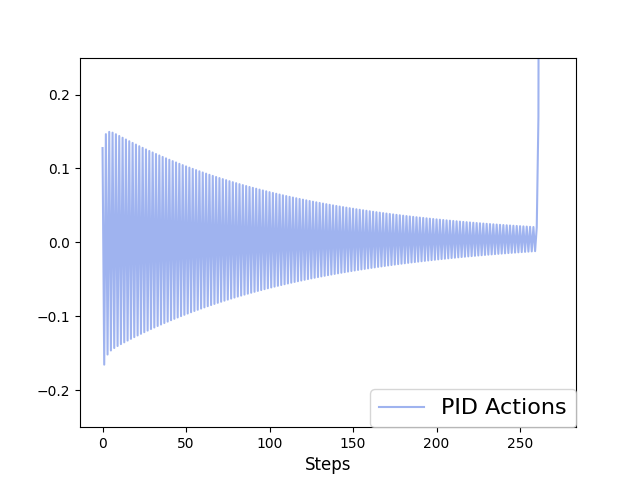
\includegraphics[width=0.3\textwidth]{ip_PID_actions}
  \caption{Actions taken by the PID controller}
  \label{fig:ip_pid_actions}
\end{figure} 

Figure \ref{fig:ip_pid} shows how the PID controller manages the pole angle and its angular velocity. The PID parameters are the following: $k_p=30,k_i=0.01,k_d=2.26$. The action of PID controller is shown in Figure \ref{fig:ip_pid_actions}. While the PID controller tries hard to converge to zero, eventually, there would be too much accumulation on the x-axis, and the equilibrium breaks down.

Based on our observations of the system, we decide to put the boundary between critical and noncritical states on the angular velocity with an absolute value of 0.4. The RL agent is free to explore with the angular velocity with an absolute value smaller than 0.4, but once it goes above this bound, the PID controller will kick in, trying to decrease the velocity back to the 0.4 bound.

\begin{figure}[H]
\centering
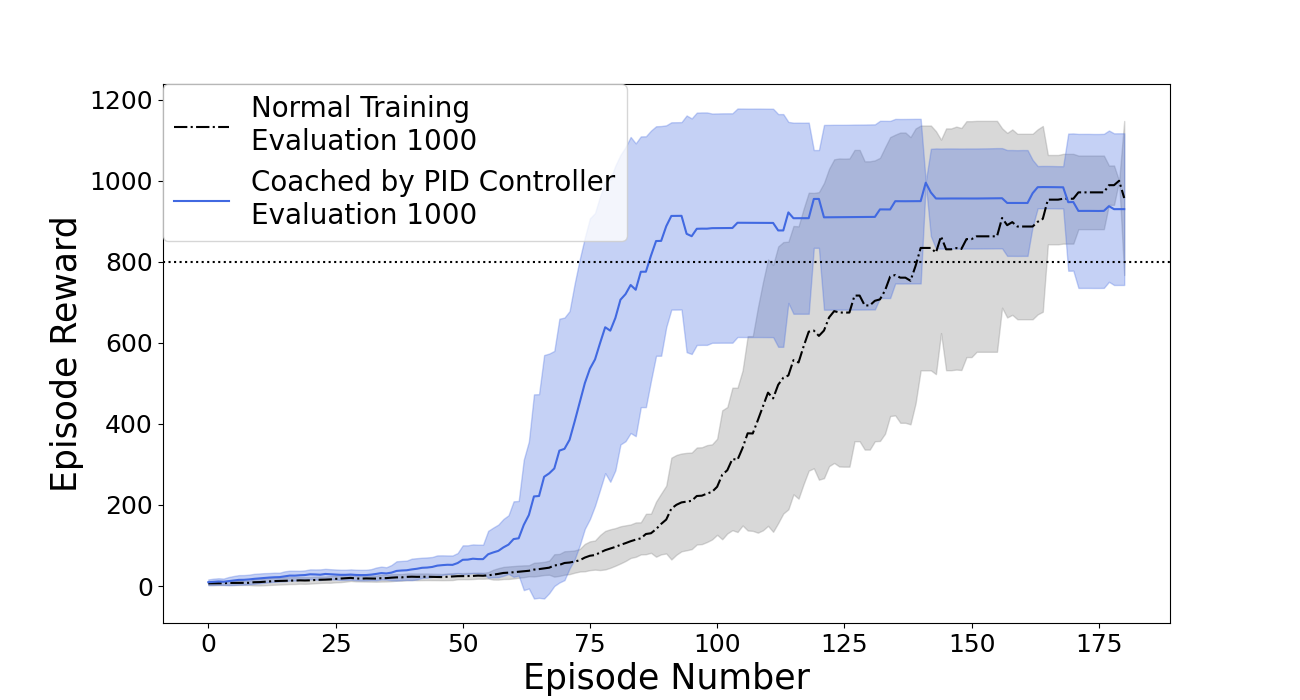
\includegraphics[width=0.5\textwidth]{ip.png}
\caption{Inverted Pendulum Experiment Result. }
\label{fig:ip_result}
\end{figure}

The experiment result is presented in Figure\ref{fig:ip_result}. The black line indicates the RL agent trained without PID coach, and the blue line indicates the agent trained with a PID coach. The points on the line are the average score over 20 episodes, and the shaded area is the standard deviation. A predetermined standard is set at a score of 800. It takes the RL agent without PID coach 160 episodes to get five consecutive scores above the standard, and it takes the RL agent with PID coach 90 episodes to do the same. PID coach results a 43.8\% acceleration in RL training. As measured by averaging over 20 episodes, it takes the RL agent without PID coach 159 episodes to go beyond 800, and it takes the RL agent with PID coach 91 episodes to do the same. PID coach results a 42.8\% acceleration in RL training. Both RL agents trained with and without PID coach pass the evaluation, and their respective average scores are presented in the upper left corner. The final performance of the RL agent is shown in Figure\ref{fig:ip_rl} and the actions taken by the RL agent is shown in Figure \ref{fig:ip_rl_actions}

\begin{figure}[H]
\centering
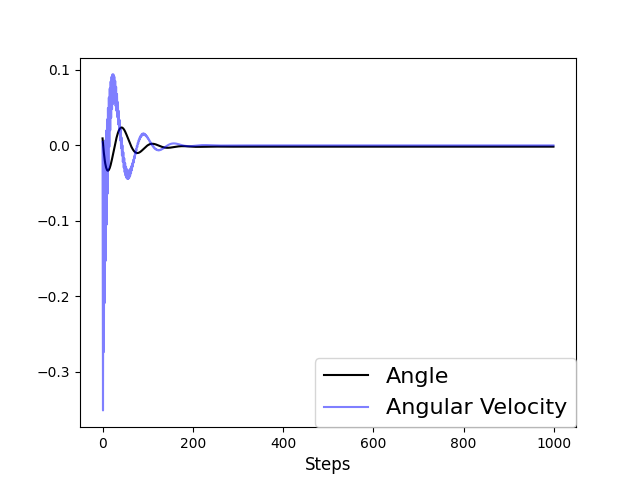
\includegraphics[width=0.3\textwidth]{ip_RL.png}
\caption{Inverted Pendulum system controlled by the RL agent. The average score achieved by the RL agent is 1000 out of 1000.}
\label{fig:ip_rl}
\end{figure}%

\begin{figure}[H]
\centering
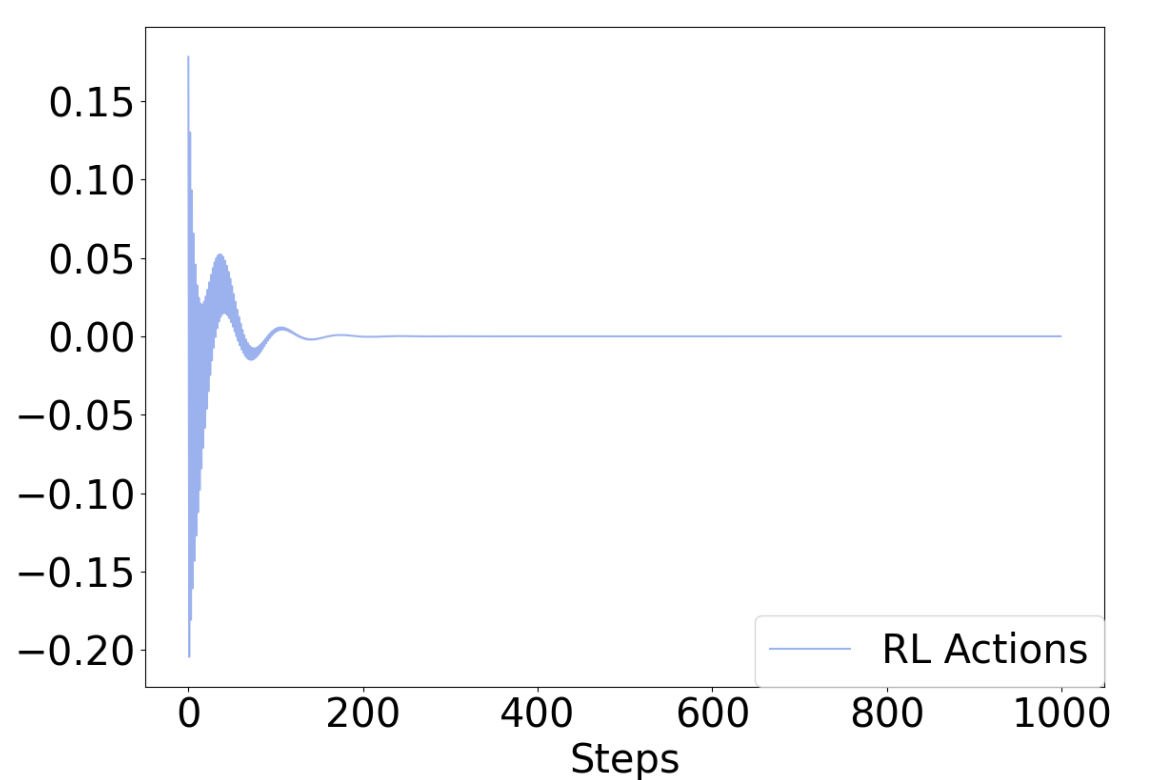
\includegraphics[width=0.3\textwidth]{ip_RL_actions.png}
\caption{Actions taken by the RL agent}
\label{fig:ip_rl_actions}
\end{figure}


\subsection{Inverted Double Pendulum}
The inverted double pendulum has observation space of the following: [x position of the cart, sin($\theta_1$), sin($\theta_2$),cos($\theta_1$),cos($\theta_2$),velocity of x, angular velocity of $\theta_1$, angular velocity of $\theta_2$, constraint force on x, constraint force on $\theta_1$, constraint force on $\theta_2$]. $\theta_1$ and $\theta_2$ are the angles of the upper and lower pole respectively. The action space for Inverted Double Pendulum is an action ranging from -1 to 1, where -1 means the actuator moves the cart to the left with maximum power and 1 means the actuator moves the cart to the right with maximum power. A score of roughly 10 points is assigned to non-terminal states, based on the velocity on the x-axis. The detailed formula for score computation can be found at the OpenAI site.

\begin{figure}[H]
\centering
\begin{subfigure}{0.3\textwidth}
\centering
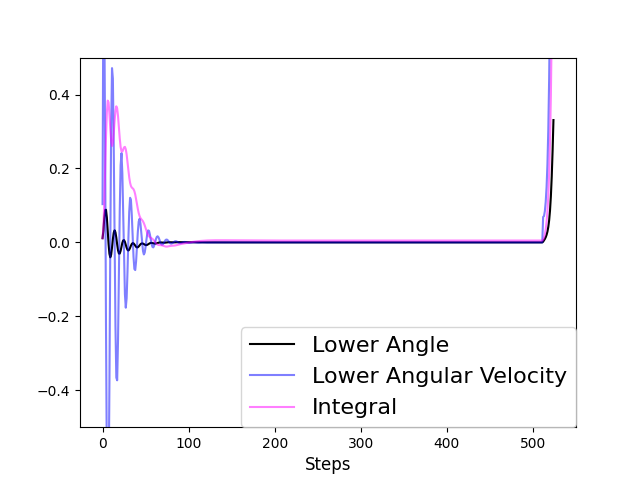
\includegraphics[width=\linewidth]{double_PID.png}
\end{subfigure}
\begin{subfigure}{0.3\textwidth}
\centering
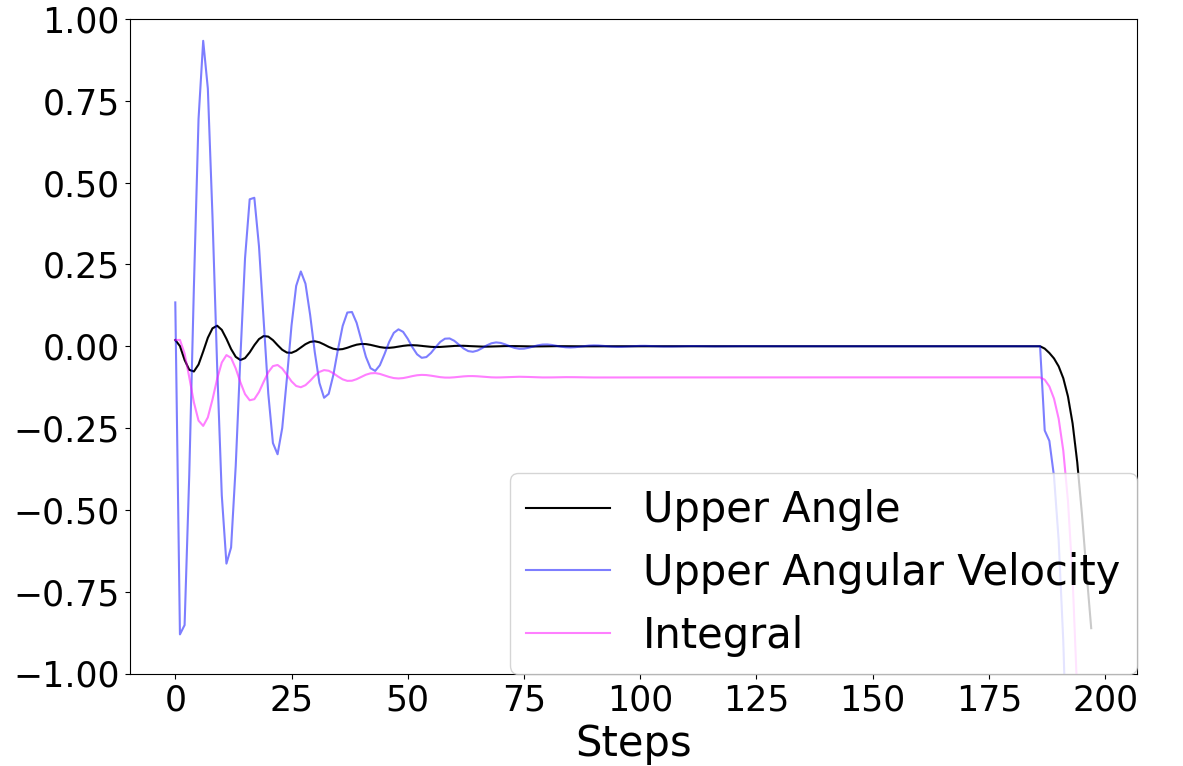
\includegraphics[width=\linewidth]{double_PID_upper.png}
\end{subfigure}
\caption{Inverted Double Pendulum system controlled the PID coach. The average score achieved by the PID controller is 1107 out of 10000. }
\label{fig:double_pid}
\end{figure}

\begin{figure}[H]
\centering
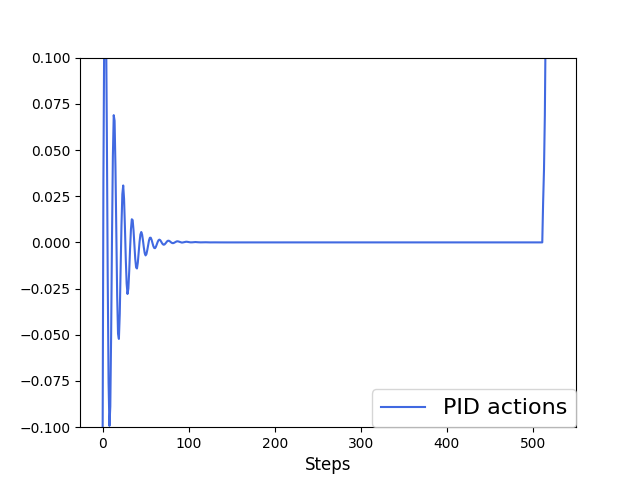
\includegraphics[width=.3\textwidth]{double_PID_actions.png}
\caption{Actions taken by the PID controller}
\label{fig:double_pid_actions}
\end{figure}

Figure\ref{fig:double_pid} shows how the PID controller manages the lower pole angle $\theta_1$ and its angular velocity $V_{\theta_1}$. The parameters for the PID coach is the following: $k_p=[-0.5,-0.5], k_i=[-0.04,-0.003], k_d=[-2.95,-0.56]$. The actions taken by the PID controller is shown in Figure \ref{fig:double_pid_actions}.The PID controller functions well until the equilibrium breaks down with too much disposition on the x-axis.

\begin{figure}[H]
\centering
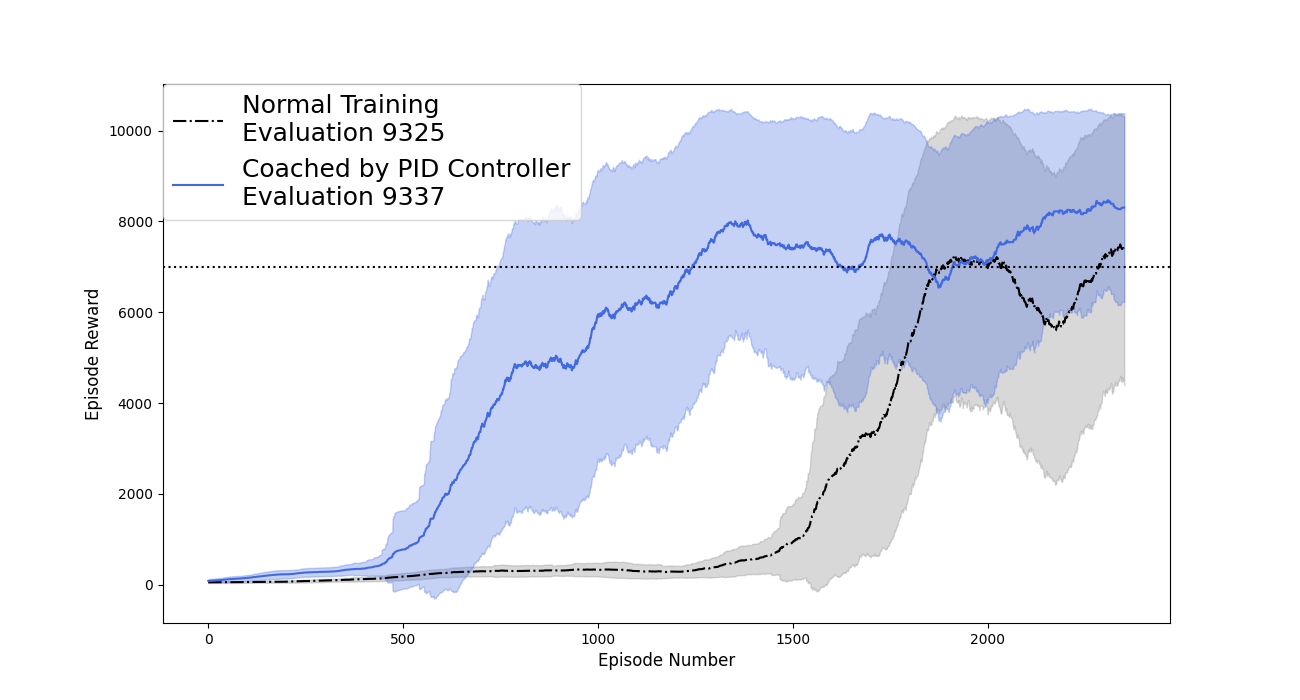
\includegraphics[width=0.5\textwidth]{double.png}
\caption{Inverted Double Pendulum Coaching Result.}
\label{fig:double_result}
\end{figure}

Based on our observation of the system, we decided to put the boundary between critical and noncritical states on the lower angle of with an absolute value of 0.2. The RL agent is free to explore with the lower angle with an absolute value smaller than 0.2, but once it goes above this bound, the PID controller will kick in, trying to nudge the lower angle back to the 0.2 bound.



\begin{figure}[H]
\centering
\begin{subfigure}{0.3\textwidth}
\centering
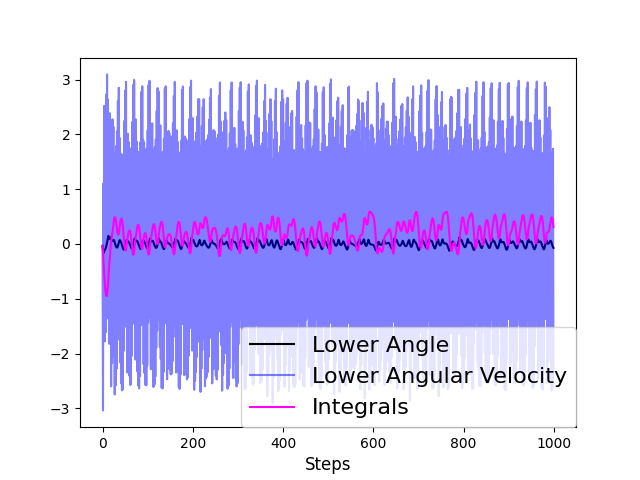
\includegraphics[width=\linewidth]{double_RL.png}
\end{subfigure}
\begin{subfigure}{0.3\textwidth}
\centering
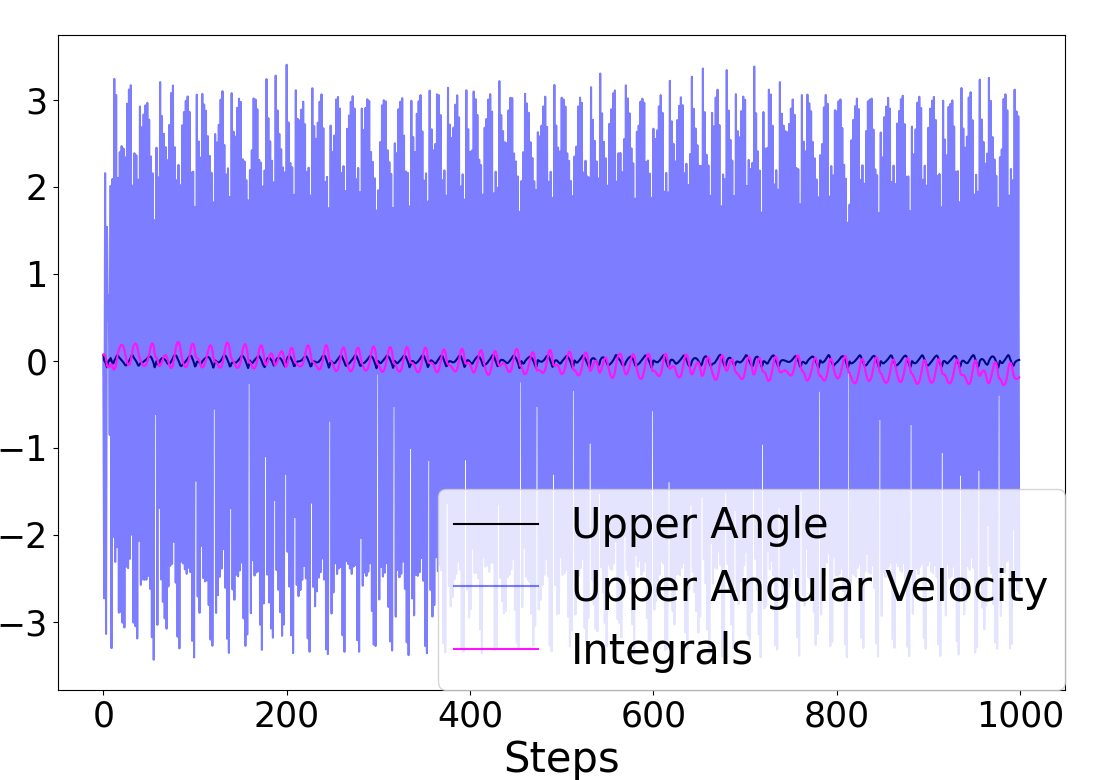
\includegraphics[width=\linewidth]{double_RL_upper.png}
\end{subfigure}
\caption{Inverted Double Pendulum system controlled the RL agent. The average score achieved by the RL agent is 9319 out of 10000. }
\label{fig:double_rl}
\end{figure}


\begin{figure}[H]
\centering
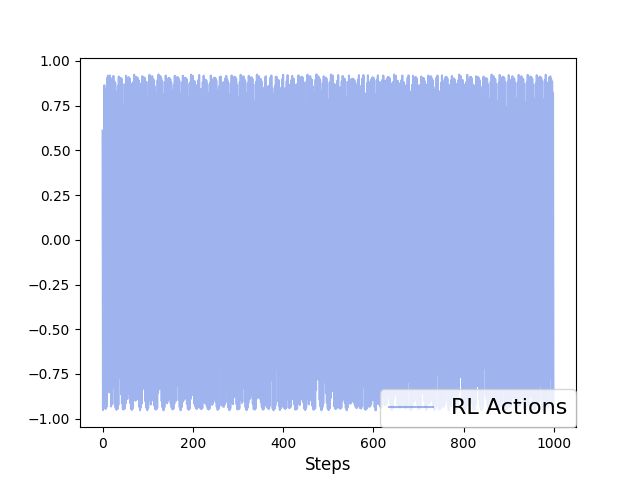
\includegraphics[width=.3\textwidth]{double_RL_actions.png}
\caption{Actions taken by the RL agent.}
\label{fig:double_rl_actions}
\end{figure}

The experiment result is presented in Figure\ref{fig:double_result}. The black line indicates the RL agent trained without PID coach, and the blue line indicates the agent trained with a PID coach. The points on the line are the average score over 200 episodes, and the shaded area is the standard deviation. A predetermined standard is set at a score of 7000. It takes the RL agent without PID coach 1909 episodes to get five consecutive scores above the standard, and it takes the RL agent with PID coach 1024 episodes to do the same. PID coach results a 46.3\% acceleration in RL training. As measured by averaging over 200 episodes, it takes RL agent without PID coach 2031 episodes to go beyond 7000, and it takes RL agent with PID coach 1391 episodes to do the same. PID coach results a 31.5\% acceleration in RL training. The discrepancy between the two measurements is stems from the fact that RL agent trained with the PID controller has a higher variance on its performance. Both agents trained with and without PID coach pass the evaluation, and their respective average scores are presented in the upper left corner. The final performance of the RL agent is shown in Figure\ref{fig:double_rl} and the actions taken by the RL agent is shown in Figure \ref{fig:double_rl_actions}.

\section{Conclusion}

This paper presents the PID controller-based coaching approach for accelerating RL training in pendulum environments. Unlike previous researches where the controllers function as teachers to the RL agents, our method emphasizes the coaching function of the controller. In both experiments, RL training is accelerated with the PID Coaches, for up to 46\%. We believe our results warrant further investigation on coaching RL agents with classic controllers. 


\bibliographystyle{IEEEtran}
\bibliography{Bibliography}
 
%% BIOGRAPHY
%% the \biography command has three parameters:
%% (1) EPS image file name without extension,
%% (2) the author's name, and (3) the texts, respectively.
%% when there is no EPS image file, just fill the first parameter with
%% {nofile}.
%% when the biography box is located
%% at vertically middle of the page apart from the text body,
%% uncomment next line.

\clearafterbiography\relax

\end{document}

